\documentclass[xetex,mathserif,serif,aspectratio=169]{beamer}

\usepackage{xltxtra}
\usepackage{color}
\usepackage{url}
\usepackage{listings}
\usepackage{fontspec}
\usepackage{geometry}
\usepackage{lastpage}
\usepackage{fancyhdr}
\usepackage{amsmath}
\usepackage{amsthm}
\usepackage{amssymb}
\usepackage{blkarray}
\usepackage{multicol}
\usepackage{relsize}
\usepackage{listings}
\usepackage{xunicode}
\usepackage{xltxtra}
\usepackage{color}
\usepackage{url}
\usefonttheme[onlymath]{serif}

\definecolor{solarized@base03}{HTML}{002B36}
\definecolor{solarized@base02}{HTML}{073642}
\definecolor{solarized@base01}{HTML}{586e75}
\definecolor{solarized@base00}{HTML}{657b83}
\definecolor{solarized@base0}{HTML}{839496}
\definecolor{solarized@base1}{HTML}{93a1a1}
\definecolor{solarized@base2}{HTML}{EEE8D5}
\definecolor{solarized@base3}{HTML}{FDF6E3}
\definecolor{solarized@yellow}{HTML}{B58900}
\definecolor{solarized@orange}{HTML}{CB4B16}
\definecolor{solarized@red}{HTML}{DC322F}
\definecolor{solarized@magenta}{HTML}{D33682}
\definecolor{solarized@violet}{HTML}{6C71C4}
\definecolor{solarized@blue}{HTML}{268BD2}
\definecolor{solarized@cyan}{HTML}{2AA198}
\definecolor{solarized@green}{HTML}{859900}
\definecolor{yaleblue}{HTML}{0E4C92}

\newcommand{\yellow}[1]{\textcolor{solarized@yellow}{#1}}
\newcommand{\orange}[1]{\textcolor{solarized@orange}{#1}}
\newcommand{\red}[1]{\textcolor{solarized@red}{#1}}
\newcommand{\magenta}[1]{\textcolor{solarized@magenta}{#1}}
\newcommand{\violet}[1]{\textcolor{solarized@violet}{#1}}
\newcommand{\blue}[1]{\textcolor{solarized@blue}{#1}}
\newcommand{\cyan}[1]{\textcolor{solarized@cyan}{#1}}
\newcommand{\green}[1]{\textcolor{solarized@green}{#1}}
\newcommand{\yblue}[1]{\textcolor{yaleblue}{#1}}
\newcommand{\base}[1]{\textcolor{solarized@base01}{#1}}


\defaultfontfeatures{Mapping=tex-text}
\hypersetup{pdfstartview={FitH}}

\newcommand{\old}[1]{\fontspec[Alternate=1,Ligatures={Common}]{Hoefler Text}\fontsize{18pt}{30pt}\selectfont #1}%
\newcommand{\oldA}[1]{\fontspec[Alternate=1,Ligatures={Common, Rare}]{Hoefler Text}\fontsize{12pt}{15pt}\selectfont #1}%
\newcommand{\oldB}[1]{\fontspec[Ligatures={Common}]{Didot}\fontsize{12pt}{15pt}\color{solarized@base02}\selectfont #1}%
\newcommand{\tfont}[1]{\fontspec[Alternate=1,Ligatures={Common}]{Hoefler Text}\fontsize{12pt}{20pt}\selectfont #1}%
\newcommand{\dfont}[1]{\fontspec[Ligatures={Common}]{Didot}\fontsize{12pt}{12pt}\selectfont #1}%

\setbeamerfont{title}{family=\old}
\setbeamerfont{author}{family=\tfont}%
\setbeamerfont{frametitle}{family=\oldA}
\setbeamerfont{date}{family=\dfont}

\setbeamertemplate{navigation symbols}{}
\setbeamertemplate{footline}[text line]{%
  \parbox{0.99\linewidth}{
    \normalsize\vspace*{-24pt}\hfill{\color{solarized@base00}\insertframenumber/\inserttotalframenumber}
  }
}


\setlength{\parindent}{0pt}
\setlength{\parskip}{12pt}

\setbeamercolor{structure}{bg=solarized@base3, fg=solarized@base02}
\setbeamercolor{titlelike}{fg=solarized@cyan}
\setbeamercolor{title}{fg=solarized@blue}
\setbeamercolor{subtitle}{fg=solarized@magenta}
\setbeamercolor{alerted text}{fg=orange}
\setbeamercolor{itemize}{fg=solarized@base02}
\setbeamercolor{background canvas}{bg=solarized@base3}
\setbeamercolor{enumerate subitem}{fg=solarized@base02}

\newcommand{\minimize}{\mathop{\mathrm{minimize}}}
\newcommand{\argmin}{\mathop{\mathrm{arg\,min}}}
\newcommand{\argmax}{\mathop{\mathrm{arg\,max}}}
\newcommand{\st}{\mathop{\mathrm{subject\,\,to}}}


\usepackage[]{algorithm2e}
\usepackage{../kbordermatrix}

\begin{document}

%%%%%%%%%%%%%%%%%%%%%%%%%%%%%%%%%%%%%%%%%%%%%%%%%%%
\begin{frame}[fragile] \frametitle{} \oldB \small

\vfill

{\fontsize{0.7cm}{0cm}\selectfont Lecture 12 \\\vspace{0.2cm} Introduction to Neural Networks}\\\vspace{0.5cm}
29 February 2016

\vspace{2cm}

\begin{minipage}{0.6\textwidth}
Taylor B. Arnold \\
Yale Statistics \\
STAT 365/665
\end{minipage}
\hfill
\begin{minipage}{0.3\textwidth}\raggedleft

\includegraphics[scale=0.3]{../yale-logo.png}
\end{minipage}%

\end{frame}

%%%%%%%%%%%%%%%%%%%%%%%%%%%%%%%%%%%%%%%%%%%%%%%%%%%
\begin{frame}[fragile] \frametitle{} \oldB \small

Notes:
\begin{itemize}
\item Problem set 4 is due this Friday (SVM implementation)
\item Problem set 5 will be posted prior to class tomorrow
  (neural net `implementation')
\end{itemize}

\end{frame}

%%%%%%%%%%%%%%%%%%%%%%%%%%%%%%%%%%%%%%%%%%%%%%%%%%%
\begin{frame}[fragile] \frametitle{} \oldB \small

\begin{center}
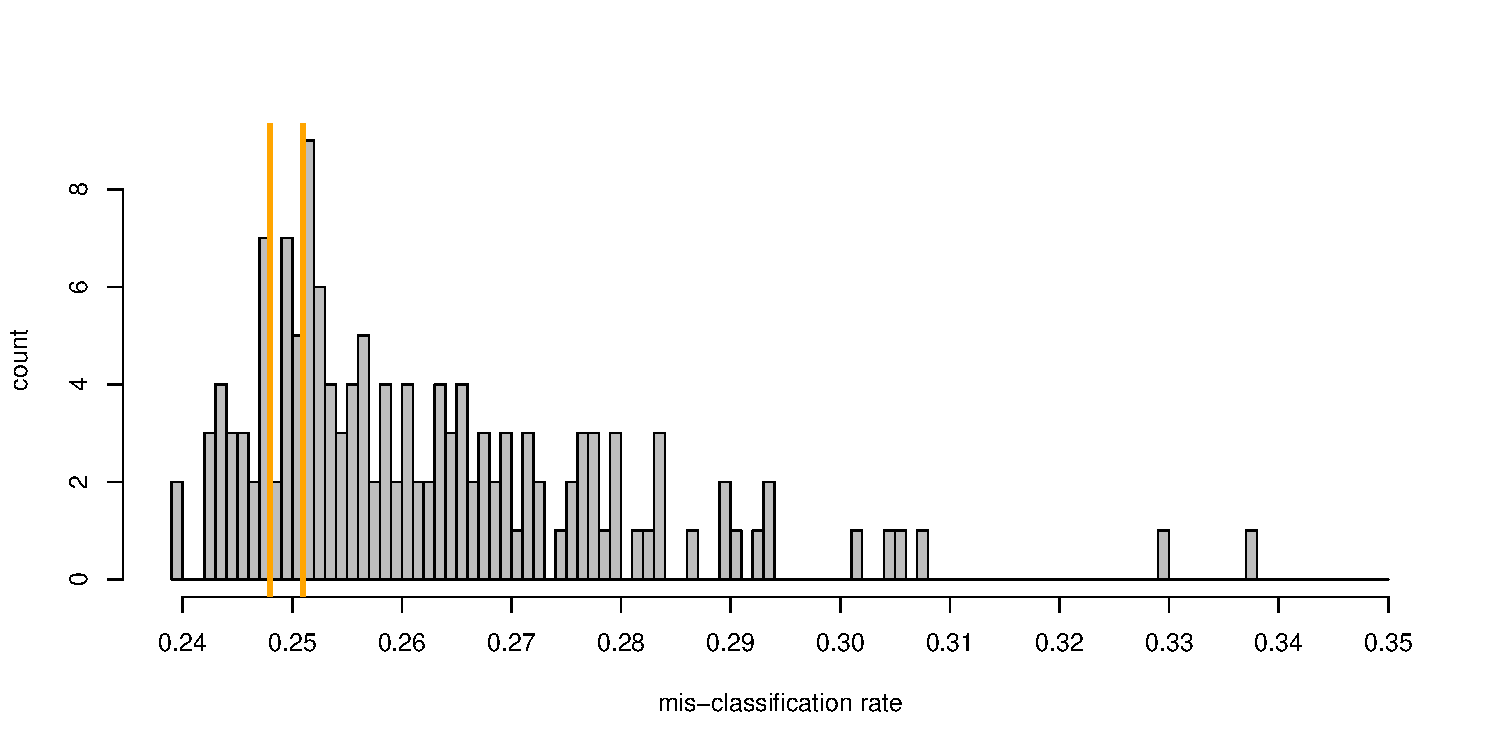
\includegraphics[width=\textwidth]{img/misRatePset03.pdf}
\end{center}

\end{frame}

%%%%%%%%%%%%%%%%%%%%%%%%%%%%%%%%%%%%%%%%%%%%%%%%%%%
\begin{frame}[fragile] \frametitle{} \oldB \small

Today
\begin{itemize}
\item Introducing neural network architecture
\item high level description of how to learn neural networks
and specific challenges in doing so
\item simulation example of SGD
\end{itemize}

\end{frame}

%%%%%%%%%%%%%%%%%%%%%%%%%%%%%%%%%%%%%%%%%%%%%%%%%%%
\begin{frame}[fragile] \frametitle{} \oldB \small

There are a large set of introductions to neural networks online. Popular
ones that I like are:

\begin{itemize}
\item Andrej Karpathy's Hacker's guide to Neural Networks: \url{http://karpathy.github.io/neuralnets/}
\item Andrej Karpathy's lecture notes: \url{http://cs231n.github.io/}
\item Geoffrey E. Hinton, Yann LeCun, and Yoshua Bengio (video; NIPS 2015): \url{http://research.microsoft.com/apps/video/default.aspx?id=259574}
\item Michael Nielsen's Neural Networks and Deep Learning: \url{http://neuralnetworksanddeeplearning.com/}
\end{itemize}

I think these are all worthwhile, and approach the subject from slightly different
angles and with different learning outcomes. I am going to (very) closely follow
Michael Nielsen's notes for the next two lectures, as I think they work the best
in lecture format and for the purposes of this course. We will then switch gears
and start following Karpathy's lecture notes in the following week.

\end{frame}

%%%%%%%%%%%%%%%%%%%%%%%%%%%%%%%%%%%%%%%%%%%%%%%%%%%
\begin{frame}[fragile] \frametitle{} \oldB \small

\yblue{\textbf{A simple decision}}

Say you want to decide whether you are going to attend a cheese festival this
upcoming weekend. There are three variables that go into your decision:
\begin{enumerate}
\item Is the weather good?
\item Does your friend want to go with you?
\item Is it near public transportation?
\end{enumerate}
We'll assume that answers to these questions are the only factors that go
into your decision.

\end{frame}

%%%%%%%%%%%%%%%%%%%%%%%%%%%%%%%%%%%%%%%%%%%%%%%%%%%
\begin{frame}[fragile] \frametitle{} \oldB \small

\yblue{\textbf{A simple decision, cont.}}

I will write the answers to these question as binary variables $x_i$, with
zero being the answer `no' and one being the answer `yes':
\begin{enumerate}
\item Is the weather good? \quad \blue{$x_1$}
\item Does your friend want to go with you?  \quad \blue{$x_2$}
\item Is it near public transportation?  \quad \blue{$x_3$}
\end{enumerate}
Now, what is an easy way to describe the decision statement resulting from
these inputs.

\end{frame}

%%%%%%%%%%%%%%%%%%%%%%%%%%%%%%%%%%%%%%%%%%%%%%%%%%%
\begin{frame}[fragile] \frametitle{} \oldB \small

\yblue{\textbf{A simple decision, cont.}}

We could determine weights $w_i$ indicating how important each feature is
to whether you would like to attend. We can then see if:
\begin{align*}
x_1 \cdot w_1 + x_2 \cdot w_2 + x_3 \cdot w_3 \geq \text{threshold}
\end{align*}
For some pre-determined threshold. If this statement is true, we would
attend the festival, and otherwise we would not.

\end{frame}

%%%%%%%%%%%%%%%%%%%%%%%%%%%%%%%%%%%%%%%%%%%%%%%%%%%
\begin{frame}[fragile] \frametitle{} \oldB \small

\yblue{\textbf{A simple decision, cont.}}

For example, if we really hated bad weather but care less about going with
our friend and public transit, we could pick the weights $6$, $2$ and $2$.

\pause With a threshold of $5$, this causes us to go if and only if the weather
is good.

\pause What happens if the threshold is decreased to $3$? What about if it is
decreased to $1$?

\end{frame}

%%%%%%%%%%%%%%%%%%%%%%%%%%%%%%%%%%%%%%%%%%%%%%%%%%%
\begin{frame}[fragile] \frametitle{} \oldB \small

\yblue{\textbf{A simple decision, cont.}}

If we define a new binary variable $y$ that represents whether we go to
the festival, we can write this variable as:
\begin{align*}
y &= \left\{ \begin{array}{c} 0, \quad x_1 \cdot w_1 + x_2 \cdot w_2 + x_3 \cdot w_3 < \text{threshold} \\
                              1, \quad x_1 \cdot w_1 + x_2 \cdot w_2 + x_3 \cdot w_3 \geq \text{threshold}
              \end{array} \right.
\end{align*}
Is this starting to look familiar yet?

\end{frame}

%%%%%%%%%%%%%%%%%%%%%%%%%%%%%%%%%%%%%%%%%%%%%%%%%%%
\begin{frame}[fragile] \frametitle{} \oldB \small

\yblue{\textbf{A simple decision, cont.}}

Now, if I rewrite this in terms of a dot product between the vector of
of all binary inputs ($x$), a vector of weights ($w$), and change the
threshold to the negative bias ($b$), we have:
\begin{align*}
y &= \left\{ \begin{array}{c} 0, \quad x \cdot w + b < 0 \\
                              1, \quad x \cdot w + b \geq 0
              \end{array} \right.
\end{align*}
So we are really just finding separating hyperplanes again, much as we
did with logistic regression and support vector machines!

\end{frame}

%%%%%%%%%%%%%%%%%%%%%%%%%%%%%%%%%%%%%%%%%%%%%%%%%%%
\begin{frame}[fragile] \frametitle{} \oldB \small

\yblue{\textbf{A perceptron}}

We can graphically represent this decision algorithm as an object that
takes $3$ binary inputs and produces a single binary output:
\begin{center}
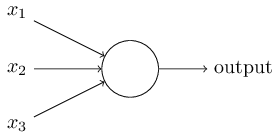
\includegraphics[width=2.5in]{img/tikz0.png}
\end{center}
This object is called a \blue{perceptron} when using the type of weighting
scheme we just developed.

\end{frame}

%%%%%%%%%%%%%%%%%%%%%%%%%%%%%%%%%%%%%%%%%%%%%%%%%%%
\begin{frame}[fragile] \frametitle{} \oldB \small

\yblue{\textbf{A network of perceptrons}}

A perceptron takes a number of binary inputs and emits a binary output.
Therefore it is easy to build a network of such perceptrons, where the
output from some perceptrons are used in the inputs of other perceptrons:
\begin{center}
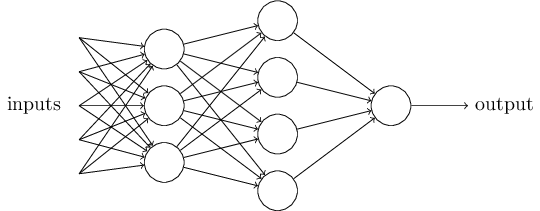
\includegraphics[width=2.8in]{img/tikz1.png}
\end{center}
Notice that some perceptrons seem to have multiple output arrows, even
though we have defined them as having only one output. This is only
meant to indicate that a single output is being sent to multiple new
perceptrons.

\end{frame}

%%%%%%%%%%%%%%%%%%%%%%%%%%%%%%%%%%%%%%%%%%%%%%%%%%%
\begin{frame}[fragile] \frametitle{} \oldB \small

\yblue{\textbf{A network of perceptrons, cont.}}

The input and outputs are typically represented as their own neurons,
with the other neurons named \blue{hidden layers}
\begin{center}
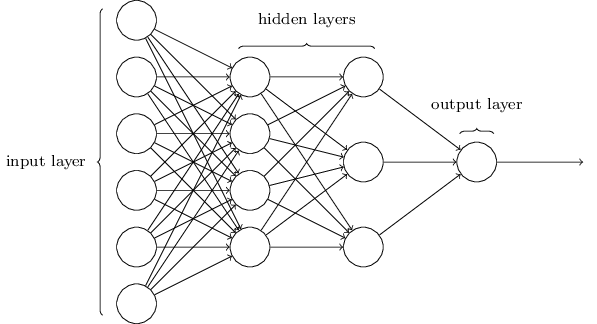
\includegraphics[width=4in]{img/tikz11.png}
\end{center}

\end{frame}

%%%%%%%%%%%%%%%%%%%%%%%%%%%%%%%%%%%%%%%%%%%%%%%%%%%
\begin{frame}[fragile] \frametitle{} \oldB \small

\yblue{\textbf{A network of perceptrons, cont.}}

The biological interpretation of a perceptron is this: when it
emits a $1$ this is equivalent to `firing' an electrical pulse,
and when it is $0$ this is when it is not firing. The bias
indicates how difficult it is for this particular node to
send out a signal.

\end{frame}

%%%%%%%%%%%%%%%%%%%%%%%%%%%%%%%%%%%%%%%%%%%%%%%%%%%
\begin{frame}[fragile] \frametitle{} \oldB \small

\begin{center}
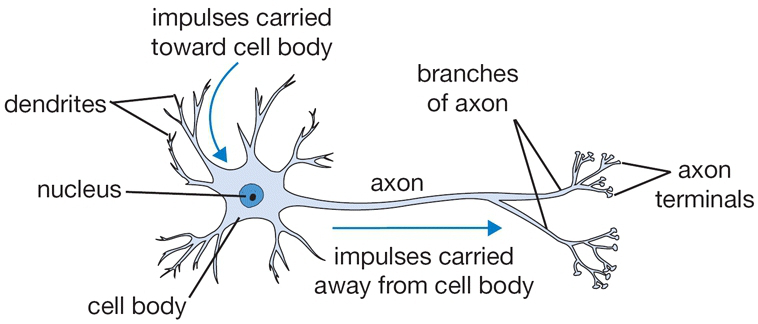
\includegraphics[height=0.7\textheight]{img/neuron.png}
\end{center}

\end{frame}

%%%%%%%%%%%%%%%%%%%%%%%%%%%%%%%%%%%%%%%%%%%%%%%%%%%
\begin{frame}[fragile] \frametitle{} \oldB \small

\begin{center}
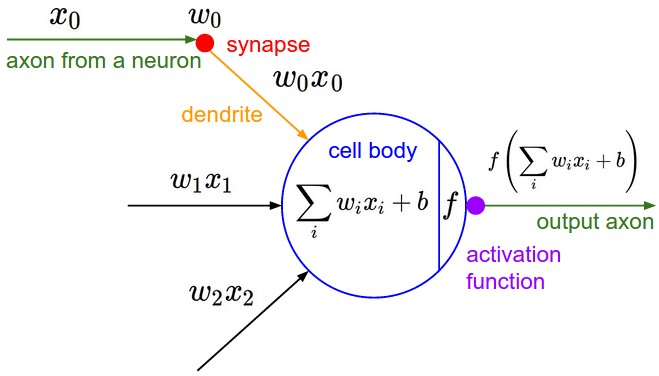
\includegraphics[height=0.7\textheight]{img/neuron_model.jpeg}
\end{center}

\end{frame}


%%%%%%%%%%%%%%%%%%%%%%%%%%%%%%%%%%%%%%%%%%%%%%%%%%%
\begin{frame}[fragile] \frametitle{} \oldB \small

\yblue{\textbf{A network of perceptrons, cont.}}

Notice that the network of nodes I have shown only sends signals
in one direction. This is called a \blue{feed-forward network}.
These are by far the most well-studied types of networks, though
we will (hopefully) have a chance to talk about recurrent neural
networks (RNNs) that allow for loops in the network. The one-directional
nature of feed-forward networks is probably the biggest difference
between artificial neural networks and their biological equivalent.

\end{frame}

%%%%%%%%%%%%%%%%%%%%%%%%%%%%%%%%%%%%%%%%%%%%%%%%%%%
\begin{frame}[fragile] \frametitle{} \oldB \small

\yblue{\textbf{Sigmoid neuron}}

An important shortcoming of a perceptron is that a small change in
the input values can cause a large change the output because each
node (or neuron) only has two possible states: $0$ or $1$. A better
solution would be to output a continuum of values, say any number
between $0$ and $1$.

Most tutorials spend a significant amount of time describing the
conceptual leap from binary outputs to a continuous output. For
us, however this should be quite straightforward.

\end{frame}

%%%%%%%%%%%%%%%%%%%%%%%%%%%%%%%%%%%%%%%%%%%%%%%%%%%
\begin{frame}[fragile] \frametitle{} \oldB \small

\yblue{\textbf{Sigmoid neuron, cont.}}

As one option, we could simply have the neuron emit the
value:
\begin{align*}
\sigma(x \cdot w + b) &= \frac{1}{1 + e^{-(x \cdot w + b)}}
\end{align*}
For a particularly positive or negative value of $x \cdot w + b$,
the result will be nearly the same as with the perceptron (i.e.,
near $0$ or $1$). For values close to the boundary of the separating
hyperplane, values near $0.5$ will be emitted.

\end{frame}

%%%%%%%%%%%%%%%%%%%%%%%%%%%%%%%%%%%%%%%%%%%%%%%%%%%
\begin{frame}[fragile] \frametitle{} \oldB \small

\yblue{\textbf{Sigmoid neuron, cont.}}

This perfectly mimics logistic regression, and in fact uses the
logit function to do so. In the neural network literature, the
logit function is called the \blue{sigmoid} function, thus leading
to the name \blue{sigmoid neuron} for a neuron that uses it's logic.

Notice that the previous restriction to binary \textit{inputs} was
not at all needed, and can be easily replaces with continuous input
without an changes needed to the formulas.

\end{frame}


%%%%%%%%%%%%%%%%%%%%%%%%%%%%%%%%%%%%%%%%%%%%%%%%%%%
\begin{frame}[fragile] \frametitle{} \oldB \small

\yblue{\textbf{Activation functions}}

In the sigmoid neuron example, the choice of what function to use
to go from $x \cdot w + b$ to an output is called the \blue{activation
function}. Using a logistic, or sigmoid, activation function has
some benefits in being able to easily take derivatives and the interpret
them using logistic regression.

Other choices have certain benefits that have recently grown in popularity.
Some of these include:
\begin{enumerate}
\item hyperbolic tan: $tanh(z) = 2 \sigma(2x) - 1$
\item rectified linear unit: $ReLU(z) = max(0, z)$
\item leaky rectified linear unit
\item maxout
\end{enumerate}
We will explore the pros and cons of these in upcoming lectures.

\end{frame}


%%%%%%%%%%%%%%%%%%%%%%%%%%%%%%%%%%%%%%%%%%%%%%%%%%%
\begin{frame}[fragile] \frametitle{} \oldB \small

\yblue{\textbf{MNIST example}}

\begin{center}
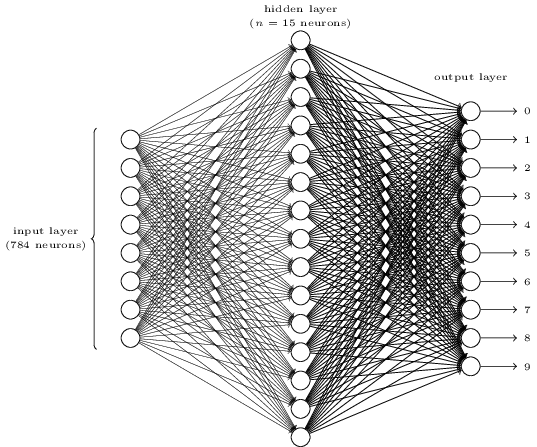
\includegraphics[height=0.8\textheight]{img/tikz12.png}
\end{center}

\end{frame}

%%%%%%%%%%%%%%%%%%%%%%%%%%%%%%%%%%%%%%%%%%%%%%%%%%%
\begin{frame}[fragile] \frametitle{} \oldB \small

\yblue{\textbf{MNIST example, classification}}

To determine which class to put a particular input into, we
look at which of the output neurons have the largest output.

\end{frame}

%%%%%%%%%%%%%%%%%%%%%%%%%%%%%%%%%%%%%%%%%%%%%%%%%%%
\begin{frame}[fragile] \frametitle{} \oldB \small

\yblue{\textbf{Learning neural networks}}

We now have an architecture that describes a neural network, but
how do we learn the weights and bias terms in the model given a
set of training data?

As an important side note, notice that with just one node, we could
define a learning algorithm which perfectly replicates a support
vector machine or logistic regression.

\end{frame}

%%%%%%%%%%%%%%%%%%%%%%%%%%%%%%%%%%%%%%%%%%%%%%%%%%%
\begin{frame}[fragile] \frametitle{} \oldB \small

\yblue{\textbf{Cost function}}

The primary set-up for learning neural networks is to define a \blue{cost
function} (also known as a \blue{loss function}) that measures how well
the network predicts outputs on the test set. The goal is to then find
a set of weights and biases that minimizes the cost.

\end{frame}

%%%%%%%%%%%%%%%%%%%%%%%%%%%%%%%%%%%%%%%%%%%%%%%%%%%
\begin{frame}[fragile] \frametitle{} \oldB \small

\yblue{\textbf{Cost function, cont.}}

One example of a cost function is just squared error loss:
\begin{align*}
C(w, b) &= \frac{1}{2n} \sum_i (y_i - \widehat{y}(x_i) )^2
\end{align*}
Or, for classification, the hinge loss:
\begin{align*}
C(w, b) &= \sum_i \left[1 - y_i \cdot \widehat{y}(x_i) \right]_{+}
\end{align*}
As with the activation functions, we'll explore the different
cost functions over the the next several weeks.

\end{frame}

%%%%%%%%%%%%%%%%%%%%%%%%%%%%%%%%%%%%%%%%%%%%%%%%%%%
\begin{frame}[fragile] \frametitle{} \oldB \small

\yblue{\textbf{Optimization problem}}

How does one actually do the optimization required in fitting neural
networks? With very few exceptions, every technique is somehow related
to \blue{gradient descent}. That is, we calculate the gradient function,
move a small amount in the opposite direction of the gradient (because
we are minimizing), and then recalculate the gradient on the new spot.

\end{frame}

%%%%%%%%%%%%%%%%%%%%%%%%%%%%%%%%%%%%%%%%%%%%%%%%%%%
\begin{frame}[fragile] \frametitle{} \oldB \small

\yblue{\textbf{Gradient descent}}

Mathematically, we can describe these updates as:
\begin{align*}
w_{k+1} &= w_k - \eta \cdot \nabla_w C \\
b_{k+1} &= b_k - \eta \cdot \nabla_b C
\end{align*}
For some value $\eta > 0$. This tuning parameter, as in gradient boosted
trees, is called the \blue{learning rate}. Too low, and learning takes a
very long time. Too small, and it is likely to have trouble finding the
true minimum (as it will keep `overshooting' it).

\end{frame}

%%%%%%%%%%%%%%%%%%%%%%%%%%%%%%%%%%%%%%%%%%%%%%%%%%%
\begin{frame}[fragile] \frametitle{} \oldB \small

\yblue{\textbf{Decomposable cost function}}

One particularly important aspect of all of the cost functions used in
neural networks is that it the are able to be decomposed over the samples.
That is:
\begin{align*}
C &= \frac{1}{n} \sum_i C_i
\end{align*}
For the individual costs $C_i$ of the $i$'th sample.

\end{frame}

%%%%%%%%%%%%%%%%%%%%%%%%%%%%%%%%%%%%%%%%%%%%%%%%%%%
\begin{frame}[fragile] \frametitle{} \oldB \small

\yblue{\textbf{Decomposable cost function, cont.}}

Consider now taking a subset $M \subseteq \{1, 2, \ldots n \}$ with size
$m$ of the training set. It would seem that we can approximate the cost function
using only this subsample of the data:
\begin{align*}
\frac{\sum_{i \in M} \nabla C_i}{m} &\approx \frac{\sum_{i=1}^n \nabla C_i}{n} \approx \nabla C
\end{align*}
So it seems that we can perhaps estimate the gradient using only a small subset
of the entire training set.

\end{frame}

%%%%%%%%%%%%%%%%%%%%%%%%%%%%%%%%%%%%%%%%%%%%%%%%%%%
\begin{frame}[fragile] \frametitle{} \oldB \small

\yblue{\textbf{Stochastic gradient descent (SGD)}}

Stochastic gradient descent uses this idea to speed up the process of doing
gradient descent. Specifically, the input data are randomly partitioned into
disjoint groups $M_1, M_2, \ldots, M_{n/m}$. We then do the following updates to
the weights (biases are done at the same time, but omitted for sake of space):
\begin{align*}
w_{k+1} &= w_k - \frac{\eta}{m} \sum_{i \in M_1} \nabla C_i \\
w_{k+2} &= w_{k+1} - \frac{\eta}{m} \sum_{i \in M_2} \nabla C_i \\
&\vdots \\
w_{k+n/m+1} &= w_{k+n/m} - \frac{\eta}{m} \sum_{i \in M_{n/m}} \nabla C_i
\end{align*}
\pause Each set $M_j$ is called a \blue{mini-batch} and going through the
entire dataset as above is called an \blue{epoch}.

\end{frame}


%%%%%%%%%%%%%%%%%%%%%%%%%%%%%%%%%%%%%%%%%%%%%%%%%%%
\begin{frame}[fragile] \frametitle{} \oldB \small

\yblue{\textbf{Stochastic gradient descent (SGD), cont.}}

You'll notice that the algorithm you need to implement in problem set 4 uses
stochastic gradient descent to find a solution the support vector machine
optimization problem.

\end{frame}

%%%%%%%%%%%%%%%%%%%%%%%%%%%%%%%%%%%%%%%%%%%%%%%%%%%
\begin{frame}[fragile] \frametitle{} \oldB \small

\yblue{\textbf{Stochastic gradient descent (SGD), cont.}}

The main tuning parameters for this technique are the \magenta{size of the
mini-batch} ($m$), the \blue{learning rate} ($\eta$) and the
\violet{number of epochs} (E) to use. Again, we will discuss these in the
upcoming weeks by way of many examples.

\textbf{Note}: Some texts refer to SGD as only describing the case with a mini-batch
size of $1$, whereas others use SGD to refer to this more generic algorithm. I believe
that the technical term for the generic algorithm is \textit{mini-batch gradient descent} (MGD),
but you will rarely hear the term.

\end{frame}

%%%%%%%%%%%%%%%%%%%%%%%%%%%%%%%%%%%%%%%%%%%%%%%%%%%
\begin{frame}[fragile] \frametitle{} \oldB \small

\yblue{\textbf{Calculating the gradient function}}

The last bit that we need in order to run SGD on a neural
network is a way to actually calculate the gradient for a
given mini-batch. This will be the sole focus of Wednesday's
lecture, when I derive the equations that allow us to calculate
the gradient in a particularly efficient way.

\end{frame}

%%%%%%%%%%%%%%%%%%%%%%%%%%%%%%%%%%%%%%%%%%%%%%%%%%%
\begin{frame}[fragile] \frametitle{} \oldB \small

\yblue{\textbf{SGD Example: OLS}}

To simulate stochastic gradient descent, consider using it to find the
ordinary least squares estimator of a multivariate regression function:
\begin{align*}
f(\beta) &= \frac{1}{n} \cdot \sum_i f_i(\beta) \\
&= \frac{1}{n} \cdot \sum_i (y_i - x_i \beta)^2 \\
&= \frac{1}{n} \cdot \sum_i (y_i^2 + \beta^t x_i^t x_i \beta - 2 y_i x_i \beta)
\end{align*}

\end{frame}

%%%%%%%%%%%%%%%%%%%%%%%%%%%%%%%%%%%%%%%%%%%%%%%%%%%
\begin{frame}[fragile] \frametitle{} \oldB \small

\yblue{\textbf{SGD Example: OLS, cont.}}

Now, the gradient of $f$ is given by:
\begin{align*}
\nabla f &= \frac{1}{n} \cdot \sum_i f_i(\beta) \\
&= \frac{1}{n} \cdot \sum_i  \nabla f_i(\beta) \\
&= \frac{2}{n} \cdot \sum_i  (x_i^t x_i \beta - x_i^t y_i)
\end{align*}
And can be approximated by:
\begin{align*}
\nabla f &\approx \frac{2}{m} \cdot \sum_{i \in M}  (x_i^t x_i \beta - x_i^t y_i)
\end{align*}
For a mini-batch $M$ of size $m$.

\end{frame}



\end{document}











